\documentclass[aspectratio=169,12pt]{beamer}
% Visual style preserved from the supplied lecture0 template.
\usepackage[T1]{fontenc}
\usepackage[utf8]{inputenc}
\usepackage{lmodern}
\usepackage{amsmath,amssymb,mathtools}
\usepackage{tikz}
\usetikzlibrary{arrows.meta,positioning,shapes.geometric}
\usepackage{array}
\usepackage{hyperref}
\usepackage{graphicx}


\definecolor{slideorange}{HTML}{FF5500}
\definecolor{bulletgreen}{HTML}{A8C9A0}
\definecolor{bulletgray}{HTML}{D9E1E8}
\definecolor{warningred}{HTML}{F12A16}
\definecolor{rulegray}{HTML}{C9CED3}

\hypersetup{
  colorlinks=true,
  urlcolor=black,
  linkcolor=black
}
\urlstyle{same}

\setbeamertemplate{navigation symbols}{}
\setbeamercolor{background canvas}{bg=white}
\setbeamercolor{normal text}{fg=black,bg=white}
\setbeamercolor{frametitle}{fg=slideorange,bg=white}
\setbeamercolor{page number in head/foot}{fg=black,bg=white}
\setbeamerfont{frametitle}{series=\bfseries,size=\LARGE}
\setbeamerfont{page number in head/foot}{size=\scriptsize}
\setbeamersize{text margin left=0.85cm,text margin right=0.85cm}

\setbeamertemplate{frametitle}{%
  \vspace*{0.18cm}%
  \begin{beamercolorbox}[wd=\paperwidth,center,sep=0.08cm]{frametitle}
    \usebeamerfont{frametitle}\insertframetitle
  \end{beamercolorbox}%
  \vspace*{0.12cm}%
}

\setbeamertemplate{footline}{%
  \leavevmode
  \begin{beamercolorbox}[wd=\paperwidth,ht=0.42cm,dp=0.15cm,center]{page number in head/foot}
    \insertframenumber
  \end{beamercolorbox}%
}

\setbeamertemplate{itemize item}{%
  \raisebox{0.15ex}{\tikz\fill[bulletgreen] (0,0) circle (0.082cm);}%
}
\setbeamertemplate{itemize subitem}{%
  \raisebox{0.15ex}{\tikz\fill[bulletgray] (0,0) circle (0.064cm);}%
}

\newcommand{\SectionSlide}[1]{%
  \begin{frame}
    \centering
    \vfill
    {\color{slideorange}\Large\bfseries #1\par}
    \vfill
  \end{frame}
}

\newcommand{\SourceNote}[1]{%
  \vfill
  \begin{flushright}
    {\scriptsize #1}
  \end{flushright}
}


\usepackage{booktabs}
\usepackage{pgfplots}
\pgfplotsset{compat=1.18}
\usetikzlibrary{matrix,fit,calc,backgrounds,intersections,patterns}

\definecolor{forestgreen}{HTML}{4C7954}
\definecolor{midgray}{HTML}{666666}
\definecolor{softorange}{HTML}{FFF0E8}
\definecolor{softgreen}{HTML}{EAF3E8}
\definecolor{softblue}{HTML}{EEF3F7}

\newcommand{\E}{\mathbb E}
\newcommand{\R}{\mathbb R}
\newcommand{\norm}[1]{\left\lVert #1\right\rVert}
\newcommand{\argmin}{\operatorname*{arg\,min}}
\newcommand{\src}[1]{\SourceNote{#1}}
\newcommand{\spaceditems}{\setlength{\itemsep}{0.25cm}}
\tikzset{
  center/.style={draw=slideorange,fill=slideorange!15,circle,minimum size=.28cm,inner sep=0pt},
  point/.style={draw=black,fill=white,circle,minimum size=.16cm,inner sep=0pt},
  softbox/.style={draw=rulegray,rounded corners=3pt,fill=softblue,align=center,inner sep=7pt},
  greenbox/.style={draw=forestgreen,rounded corners=3pt,fill=softgreen,align=center,inner sep=7pt},
  orangebox/.style={draw=slideorange,rounded corners=3pt,fill=softorange,align=center,inner sep=7pt},
  flow/.style={-{Latex[length=2.5mm]},line width=.8pt},
  thinflow/.style={-{Latex[length=2mm]},line width=.6pt},
}

\hypersetup{pdftitle={K-means Clustering},pdfauthor={Zihan Zhang},pdfsubject={COMP 5212 Machine Learning}}
\pdfstringdefDisableCommands{\def\translate#1{#1}}

\newcommand{\SectionSlideN}[2]{%
  \begin{frame}
    \centering
    \vfill
    {\color{slideorange}\fontsize{29}{34}\selectfont\bfseries #1\par}
    \vspace{0.38cm}
    {\color{midgray}\fontsize{16}{21}\selectfont #2\par}
    \vfill
  \end{frame}
}

\begin{document}

\begin{frame}
	\begin{tikzpicture}[remember picture, overlay]
		\node[anchor=north west, inner sep=10pt] at (current page.north west)
		{
\includegraphics[width=6cm]{../source/logo.png}};
	\end{tikzpicture}
	
	\centering
	\vspace*{1.15cm}
	{\fontsize{28}{32}\selectfont COMP 5212\par}
	\vspace{0.35cm}
	{\fontsize{30}{33}\selectfont Machine Learning\par}
	\vspace{0.75cm}
	{\Large Instructor: Zihan Zhang\par}
	\vspace{0.35cm}
	{\large Lecture 8: K-means Clustering\par}
	
\end{frame}

\begin{frame}{Learning Goals}
  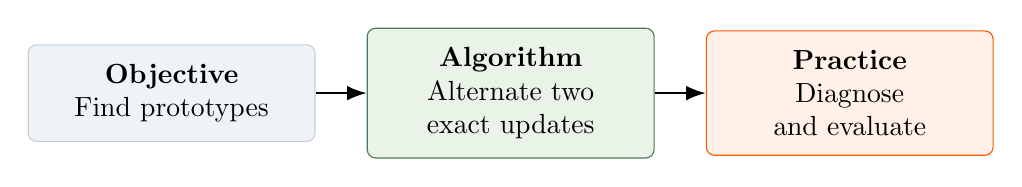
\begin{tikzpicture}[node distance=.65cm]
    \node[softbox,text width=3.15cm] (obj) {\textbf{Objective}\par Find prototypes};
    \node[greenbox,text width=3.15cm,right=of obj] (alg) {\textbf{Algorithm}\par Alternate two exact updates};
    \node[orangebox,text width=3.15cm,right=of alg] (use) {\textbf{Practice}\par Diagnose and evaluate};
    \draw[flow] (obj)--(alg); \draw[flow] (alg)--(use);
  \end{tikzpicture}
  \vspace{.45cm}
  \begin{itemize}\setlength{\itemsep}{.23cm}
    \item Justify squared error and derive the two Lloyd updates;
    \item Distinguish local-optimum facts from approximation guarantees;
    \item Choose preprocessing, $K$, and evaluation checks;
    \item Use a Johnson--Lindenstrauss projection to reduce dimension
  \end{itemize}
\end{frame}

\SectionSlideN{Motivation and Objective}

% 3 ---------------------------------------------------------------------------



\definecolor{kmOrange}{HTML}{C88753}
\definecolor{kmLime}{HTML}{9BCB53}
\definecolor{kmBlue}{HTML}{5A9DCC}
\definecolor{kmPurple}{HTML}{8054C7}
\definecolor{kmGreen}{HTML}{58B978}
\definecolor{kmPink}{HTML}{C84D9A}

\newcommand{\KmeansCloud}[6]{%
	\foreach \x/\y in {
		0.8/6.3,1.6/6.45,2.1/6.8,2.6/6.1,
		1.8/6.0,2.9/6.35,2.4/5.85,1.2/6.0,
		2.7/6.7,1.9/6.25,2.3/6.55,2.8/5.75,
		1.5/5.8,2.1/5.7,2.9/6.05
	}{\fill[#1] (\x,\y) circle (2.6pt);}
	
	\foreach \x/\y in {
		9.0/6.6,9.4/6.2,9.8/6.8,10.2/6.35,
		10.6/6.55,9.6/6.0,10.0/6.1,10.8/6.7,
		9.3/5.85,9.9/6.45,10.4/6.05,9.7/6.55,
		10.9/6.35,9.5/6.9,10.2/6.95
	}{\fill[#2] (\x,\y) circle (2.6pt);}
	
	\foreach \x/\y in {
		7.5/3.2,8.0/2.9,8.4/3.5,8.9/3.1,
		9.2/2.7,8.2/2.3,7.8/2.4,8.7/2.6,
		9.0/3.7,7.7/2.0,8.4/2.8,8.9/2.2,
		7.9/3.8,8.6/3.3,9.4/2.9
	}{\fill[#3] (\x,\y) circle (2.6pt);}
	
	\foreach \x/\y in {
		10.3/4.1,10.8/4.4,11.1/3.8,10.6/3.5,
		11.4/4.0,10.9/3.3,11.5/3.7,10.5/3.9,
		11.0/4.6,10.2/3.6,11.3/4.2
	}{\fill[#4] (\x,\y) circle (2.6pt);}
	
	\foreach \x/\y in {
		9.5/2.2,9.8/2.5,10.2/2.0,10.6/2.4,
		10.9/1.9,9.9/1.8,10.4/2.2,11.1/2.1,
		9.7/1.6,10.7/1.7,10.3/2.7,9.4/1.9
	}{\fill[#5] (\x,\y) circle (2.6pt);}
	
	\foreach \x/\y in {
		3.2/2.6,3.8/2.0,4.2/2.4,4.7/1.7,
		5.1/1.9,5.6/1.4,6.0/1.8,4.3/1.5,
		3.6/1.8,4.8/2.2,5.4/1.3,5.8/2.1,
		4.0/2.8,4.9/1.1,5.5/1.7,6.2/1.6,
		3.4/1.4
	}{\fill[#6] (\x,\y) circle (2.6pt);}
}

\newcommand{\KmeansCenters}{%
	\foreach \x/\y in {
		2.35/6.25,
		9.75/6.4,
		8.55/2.75,
		10.85/3.85,
		10.25/2.25,
		4.75/1.85
	}{
		\draw[black,line width=.9pt] (\x,\y) circle (.16);
		\draw[black,line width=.9pt]
		(\x-.11,\y-.11)--(\x+.11,\y+.11)
		(\x-.11,\y+.11)--(\x+.11,\y-.11);
	}
}

% Before coloring



% Before coloring

\definecolor{clusterblue}{HTML}{5A9DCC}

\begin{frame}{User-Behavior Clustering}
	\small
	\begin{center}
		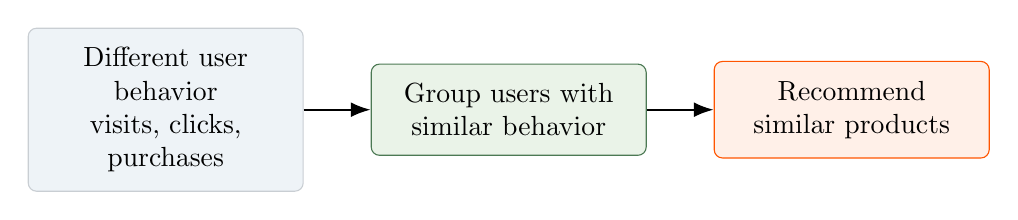
\begin{tikzpicture}[node distance=.85cm]
			\node[softbox,text width=3.0cm] (behavior)
			{Different user behavior\\visits, clicks, purchases};
			
			\node[greenbox,text width=3.0cm,right=of behavior] (groups)
			{Group users with similar behavior};
			
			\node[orangebox,text width=3.0cm,right=of groups] (recommend)
			{Recommend similar products};
			
			\draw[flow] (behavior)--(groups);
			\draw[flow] (groups)--(recommend);
		\end{tikzpicture}
	\end{center}
	
	\vspace{.35cm}
	
	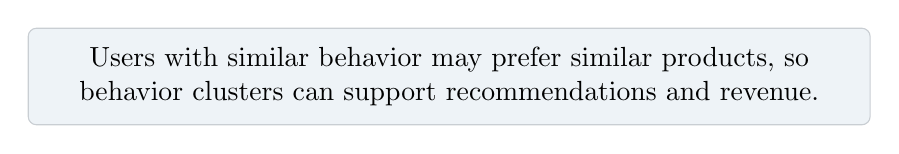
\begin{tikzpicture}
		\node[softbox,text width=10.2cm]
		{Users with similar behavior may prefer similar products, so behavior clusters can support recommendations and revenue.};
	\end{tikzpicture}
	\begin{itemize}
		\item Why not classification?
	\end{itemize}
\end{frame}


\begin{frame}{A Clustering Example}
	\centering
	\resizebox{.80\textwidth}{!}{%
		\begin{tikzpicture}[x=.9cm,y=.78cm]
			\draw[rulegray!70,line width=1pt] (0,0)--(12.2,0);
			\draw[rulegray!70,line width=1pt] (0,0)--(0,7.5);
			
			\KmeansCloud
			{black}{black}{black}
			{black}{black}{black}
		\end{tikzpicture}
	}
\end{frame}

% After coloring
\begin{frame}{A Clustering Example}
	\centering
	\resizebox{.80\textwidth}{!}{%
		\begin{tikzpicture}[x=.9cm,y=.78cm]
			\draw[rulegray!70,line width=1pt] (0,0)--(12.2,0);
			\draw[rulegray!70,line width=1pt] (0,0)--(0,7.5);
			
			\KmeansCloud
			{kmOrange}{kmLime}{kmBlue}
			{kmPurple}{kmGreen}{kmPink}
			
			\KmeansCenters
		\end{tikzpicture}
	}
\end{frame}


\begin{frame}{What Is the Object We Want to Learn?}
  \begin{columns}[T,onlytextwidth]
    \column{.48\textwidth}
      \textbf{Observed data}
      \[
        x_1,\ldots,x_n\in\R^d.
      \]
      \vspace{.08cm}
      \textbf{Unknown structure}
      \[
        C_1,\ldots,C_K\quad\text{a partition of }\{1,\ldots,n\}.
      \]
    \column{.46\textwidth}
      For each proposed cluster $C_k$, compute its coordinate-wise mean
      \[
        \bar x_{C_k}=\frac{1}{|C_k|}\sum_{i\in C_k}x_i.
      \]
      \begin{itemize}\spaceditems
        \item Labels are not supplied;
        \item $K$ is chosen before fitting;
        \item compactness is measured in the selected feature geometry.
      \end{itemize}
  \end{columns}
  \vspace{.28cm}
  \centering
  \textbf{Goal: find a partition whose members are close to their own cluster mean.}
\end{frame}

% 4 ---------------------------------------------------------------------------
\begin{frame}{Why Use Squared Error?}
  \small
  For a partition $C_1,\ldots,C_K$, define the empirical within-cluster error directly from the means:
  \[
    \operatorname{SSE}(C_1,\ldots,C_K)
    =\sum_{k=1}^{K}\sum_{i\in C_k}\norm{x_i-\bar x_{C_k}}^2.
  \]
  \vspace{.08cm}
\begin{itemize}
	\item  Robust to general noise assumptions;
	\item  Feasible to dimension reductions.
\end{itemize}
\end{frame}

% 5 -----------------------------------------------------------------

% 6 ---------------------------------------------------------------------------



\SectionSlideN{The Algorithm}

% 7 ---------------------------------------------------------------------------
\begin{frame}{Lloyd's Algorithm}
  \begin{enumerate}\spaceditems
    \item Choose $K$ initial centers $\mu_1,\ldots,\mu_K$.
    \item \textbf{Assignment:} $z_i\leftarrow\argmin_k\norm{x_i-\mu_k}^2$.
    \item \textbf{Update:} $\mu_k\leftarrow\frac{1}{|C_k|}\sum_{i:z_i=k}x_i$.
    \item Repeat until assignments, centers, or $J$ stop changing.
  \end{enumerate}
\end{frame}

% 8 ---------------------------------------------------------------------------
\begin{frame}{A 2-D K-means Demo in the Browser}
  \centering
  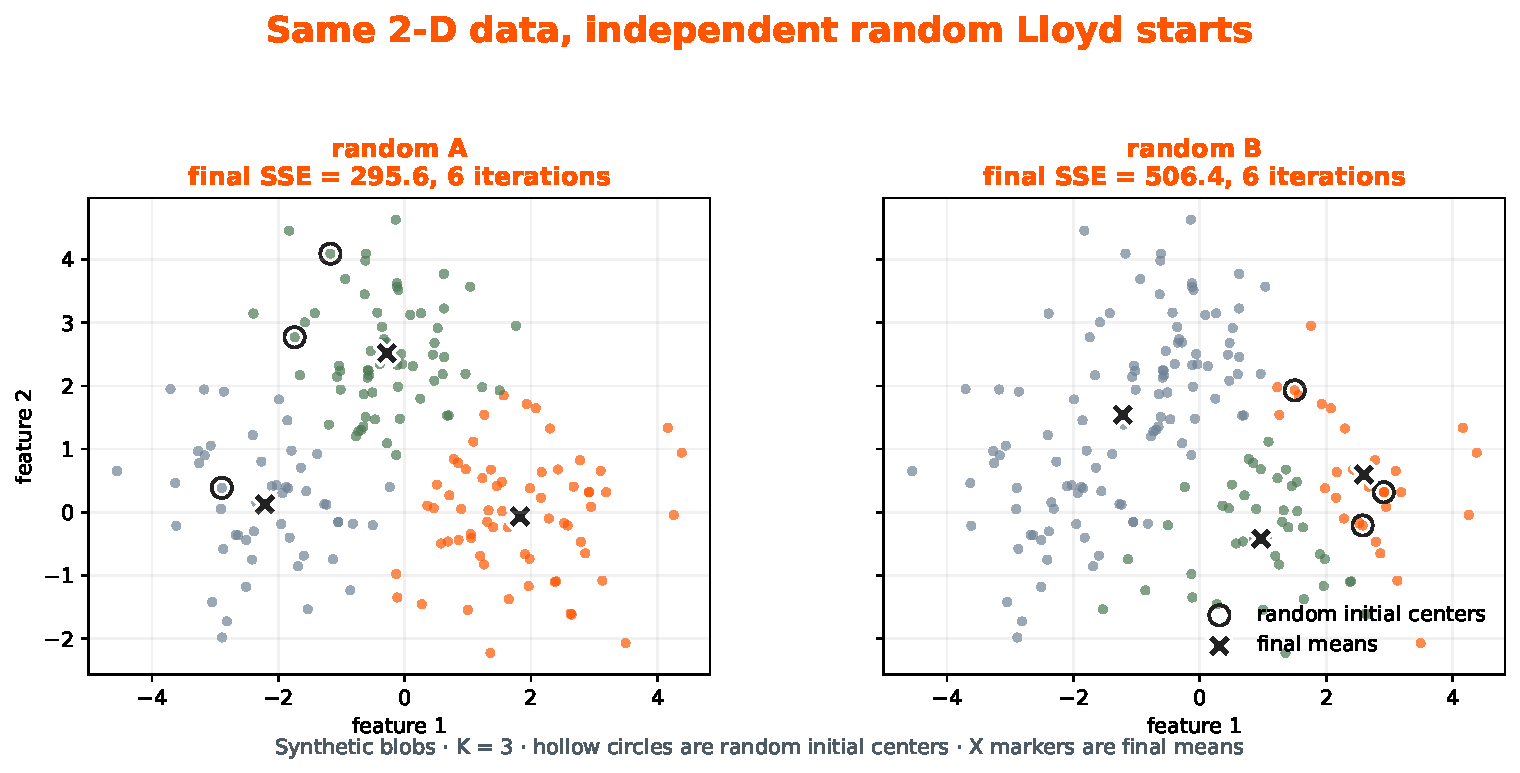
\includegraphics[width=.80\textwidth]{assets/fig_initialization_demo.pdf}
  \vspace{.01cm}
\end{frame}

% 9 ---------------------------------------------------------------------------
\begin{frame}{The Assignment Step Creates Voronoi Cells}
  \begin{columns}[c,onlytextwidth]
    \column{.52\textwidth}
      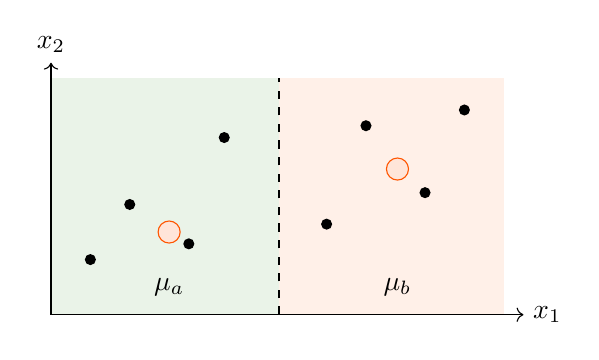
\begin{tikzpicture}[x=.50cm,y=.50cm]
        \fill[softgreen] (0,0) -- (5.8,0) -- (5.8,6) -- (0,6) -- cycle;
        \fill[softorange] (5.8,0) -- (11.5,0) -- (11.5,6) -- (5.8,6) -- cycle;
        \draw[->] (0,0)--(12,0) node[right]{$x_1$};
        \draw[->] (0,0)--(0,6.4) node[above]{$x_2$};
        \draw[dashed,thick] (5.8,0)--(5.8,6);
        \node[center] at (3,2.1) {};
        \node[center] at (8.8,3.7) {};
        \node at (3,.7) {$\mu_a$};\node at (8.8,.7) {$\mu_b$};
        \foreach \x/\y in {1/1.4,2/2.8,3.5/1.8,4.4/4.5,7/2.3,8/4.8,9.5/3.1,10.5/5.2}{\fill[black] (\x,\y) circle (2pt);}
      \end{tikzpicture}
    \column{.42\textwidth}
      A point belongs to the center with the smaller squared distance.
      \[
        \norm{x-\mu_a}^2\le \norm{x-\mu_b}^2.
      \]
      \pause
      The boundary is a hyperplane; K-means \textcolor{red}{cannot} express arbitrary non-convex cells.
  \end{columns}
\end{frame}

% 10 --------------------------------------------------------------------------
\begin{frame}{Why Does Lloyd's Objective Decrease?}
  \begin{columns}[T,onlytextwidth]
    \column{.47\textwidth}
      \textbf{Assignment step}
      \[
        J(z^{t+1},\mu^t)\le J(z^t,\mu^t).
      \]
      Each sample chooses its nearest current center.
    \column{.47\textwidth}
      \textbf{Update step}
      \[
        J(z^{t+1},\mu^{t+1})\le J(z^{t+1},\mu^t).
      \]
      Each center becomes the best mean for its current cluster.
  \end{columns}
  \pause
  \vspace{.35cm}
  \[
    J^0\ge J^1\ge J^2\ge\cdots\ge0.
  \]
  \centering
  Monotone descent gives a fixed point, not a guarantee of the global optimum.
\end{frame}


\SectionSlideN{Theory and Practice}

% 11 --------------------------------------------------------------------------
\begin{frame}{What Does a Lloyd Fixed Point Guarantee?}
  \footnotesize
  \begin{columns}[T,onlytextwidth]
    \column{.46\textwidth}
      \textbf{For arbitrary initialization}
      \begin{itemize}\setlength{\itemsep}{.06cm}
        \item With deterministic tie-breaking, SSE is non-increasing and the finite assignment set leads to a fixed point.
        \item A fixed point is stationary under the two Lloyd updates, not globally optimal.
        \item Arbitrary Lloyd starts have \textcolor{red}{no} finite worst-case approximation ratio.
      \end{itemize}
    \column{.46\textwidth}
      \textbf{What initialization can add}
      \begin{itemize}\setlength{\itemsep}{.06cm}
        \item k-means++ [AV2007] gives
        \[
          \E[J_{\mathrm{init}}]\le 8(\ln K+2)\,J^*.
        \]
        \item Lloyd iterations only decrease $\phi$, so the same expected upper bound holds for the final run.
        \item Computing $J^*$ is l NP-hard in the general case.
      \end{itemize}
  \end{columns}
  \vspace{0.5cm}
  \scriptsize [AV2007]  k-means++: The Advantages of Careful Seeding. David Arthur and Sergei Vassilvitskii, SODA 2007, pp. 1027–1035.
\end{frame}

% 12 ------------------------------------------------------------------

% 13 --------------------------------------------------------------------------
\begin{frame}{Initialization Is Part of the Algorithm}
  \begin{columns}[T,onlytextwidth]
    \column{.47\textwidth}
      \textbf{Random starts}
      \begin{itemize}\spaceditems
        \item Simple, but centers may start together.
        \item A single seed can be misleading.
      \end{itemize}
    \column{.47\textwidth}
      \textbf{k-means++}
      \begin{itemize}\spaceditems
        \item Choose the first center at random.
        \item Sample later centers with probability proportional to squared distance from the current set.
      \end{itemize}
  \end{columns}
  \pause
  \vspace{.5cm}
  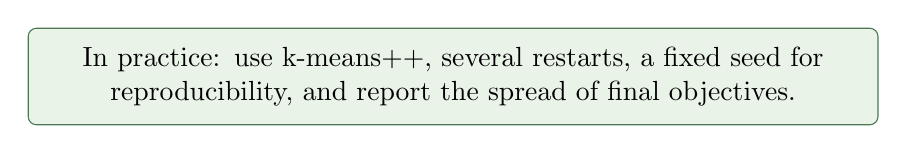
\begin{tikzpicture}
    \node[greenbox,text width=10.3cm] {In practice: use k-means++, several restarts, a fixed seed for reproducibility, and report the spread of final objectives.};
  \end{tikzpicture}
\end{frame}

% 12 --------------------------------------------------------------------------
\begin{frame}{Implementation Details Change the Result}

      \begin{itemize}\spaceditems
        \item Standardize or transform features before measuring distances.
        \item Decide how to handle missing values and empty clusters.
        \item Remove or robustly treat influential outliers.
           \item Use MiniBatchKMeans when one full pass is too expensive.
      \end{itemize}

\end{frame}

% 13 ------------------------------------------------------------------
% 14 --------------------------------------------------------------------------
\begin{frame}{How Should We Choose $K$?}
  \begin{columns}[T,onlytextwidth]
    \column{.46\textwidth}
      \textbf{Inertia}
      \[
        \operatorname{inertia}(K)=\min_{z,\mu}J(z,\mu).
      \]
      It never increases as $K$ grows.
    \column{.46\textwidth}
      \textbf{Silhouette}
      \[
        s_i=\frac{b_i-a_i}{\max(a_i,b_i)}.
      \]
      Compare within-cluster and nearest-other-cluster distances.
  \end{columns}
  \vspace{.5cm}
  \small
  \begin{itemize}
  	\item $a_i$:  the average distance to the datapoints within the same clique  $\frac{1}{ |C_i|-1} \sum_{j\in C_i, j\neq i} \|x_i - x_i\|$
  	\item $b_i$:  the minimal average distance to a neighbor clique $\min_{C\neq C_i} \frac{1}{|C|} \sum_{j\in C} \| x_i- x_j\|$.
  \end{itemize}
\end{frame}

% 15 --------------------------------------------------------------------------
\begin{frame}{A Low Inertia Is Not Always Good}
  \begin{columns}[c,onlytextwidth]
    \column{.48\textwidth}
      \begin{tikzpicture}[x=.46cm,y=.42cm]
        \draw[->] (0,0)--(8.8,0) node[right]{$K$};
        \draw[->] (0,0)--(0,6.1) node[above]{inertia};
        \draw[thick,forestgreen] plot[smooth] coordinates {(1,5.5)(2,3.2)(3,2.2)(4,1.8)(5,1.6)(6,1.48)(7,1.4)(8,1.34)};
      \end{tikzpicture}
    \column{.46\textwidth}
      \begin{itemize}\spaceditems
        \item Increasing $K$ always improves the training objective.
        \item A stable cluster across seeds or resamples is more credible.
        \item A useful cluster must have an interpretable consequence.
      \end{itemize}
  \end{columns}
\end{frame}

% 16 --------------------------------------------------------------------------
\begin{frame}{Failure Gallery: The Geometry Is the Model}
  \begin{columns}[T,onlytextwidth]
    \column{.31\textwidth}
      \centering
      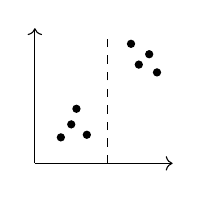
\begin{tikzpicture}[x=.33cm,y=.33cm]
        \draw[->] (0,0)--(5.3,0);\draw[->] (0,0)--(0,5.2);
        \foreach \x/\y in {1/1,1.4/1.5,2/1.1,1.6/2.1,4/3.8,4.4/4.2,3.7/4.6,4.7/3.5}{\fill[black] (\x,\y) circle (1.5pt);}
        \draw[dashed] (2.8,0)--(2.8,5);
      \end{tikzpicture}
      \par\small Well-separated blobs
    \column{.31\textwidth}
      \centering
      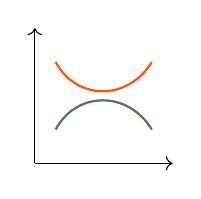
\begin{tikzpicture}[x=.33cm,y=.33cm]
        \draw[->] (0,0)--(5.3,0);\draw[->] (0,0)--(0,5.2);
        \draw[thick,forestgreen] (0.8,1.3) .. controls (1.6,2.8) and (3.6,2.8) .. (4.5,1.3);
        \draw[thick,slideorange] (0.8,3.9) .. controls (1.6,2.4) and (3.6,2.4) .. (4.5,3.9);
      \end{tikzpicture}
      \par\small Non-convex structure
    \column{.31\textwidth}
      \centering
      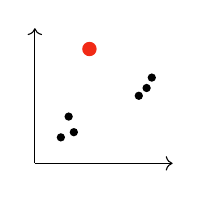
\begin{tikzpicture}[x=.33cm,y=.33cm]
        \draw[->] (0,0)--(5.3,0);\draw[->] (0,0)--(0,5.2);
        \foreach \x/\y in {1/1,1.5/1.2,1.3/1.8,4/2.6,4.3/2.9,4.5/3.3,2.1/4.4}{\fill[black] (\x,\y) circle (1.5pt);}
        \fill[warningred] (2.1,4.4) circle (2.6pt);
      \end{tikzpicture}
      \par\small Unequal density and outliers
  \end{columns}
  \vspace{.45cm}
  \centering
  When K-means fails, ask whether the distance, scale, $K$, or cluster shape is mismatched to the data.
\end{frame}

% 17 --------------------------------------------------------------------------
\begin{frame}{Complexity and Scaling to Larger Data}
  Total computational cost $O(nKdt)$.
  \begin{itemize}
  	\item $n$: the size of dataset;
  	\item $K$: the number of clusters;
  	\item $d$: feature dimension;
  	\item $t$:  number of iteration steps.
  \end{itemize}
  \vspace{0.3cm}
  \pause
  Approaches for scaling up
      \begin{itemize}\spaceditems
        \item Mini-batches reduce the cost of each update.
        \item Sparse or approximate distance routines reduce memory pressure.
      \end{itemize}
\end{frame}


\SectionSlideN{Applications}

% 18 --------------------------------------------------------------------------
% 19 --------------------------------------------------------------------------
\begin{frame}{Application: K-means as an IVF Search Coarse Quantizer}
  \small
  \begin{center}
    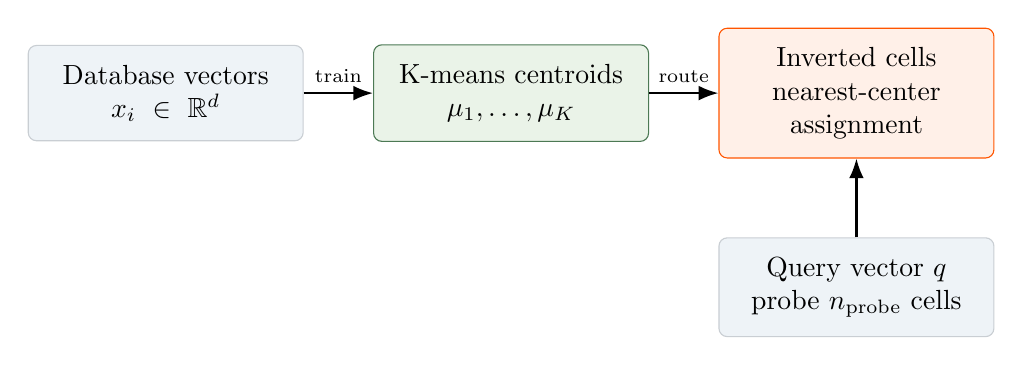
\begin{tikzpicture}[node distance=.88cm]
      \node[softbox,text width=3.0cm] (vec) {Database vectors\\$x_i\in\R^d$};
      \node[greenbox,text width=3.0cm,right=of vec] (cent) {K-means centroids\\$\mu_1,\ldots,\mu_K$};
      \node[orangebox,text width=3.0cm,right=of cent] (cell) {Inverted cells\\nearest-center assignment};
      \draw[flow] (vec)--node[above,font=\scriptsize]{train}(cent);
      \draw[flow] (cent)--node[above,font=\scriptsize]{route}(cell);
      \node[softbox,text width=3.0cm,below=1.0cm of cell] (query) {Query vector $q$\\probe $n_{\mathrm{probe}}$ cells};
      \draw[flow] (query)--(cell);
    \end{tikzpicture}
  \end{center}
  \vspace{-.23cm}
  \begin{itemize}\setlength{\itemsep}{.03cm}
    \item $x_i$ is a stored embedding or feature vector; a cluster is one coarse inverted cell.
    \item A query probes selected cells, then exact distances rerank candidates; $n_{\mathrm{probe}}$ trades recall against latency.
  \end{itemize}
\end{frame}

% 20 --------------------------------------------------------------------------
\begin{frame}{Experiments Expose the Preprocessing Assumptions}
  \centering
  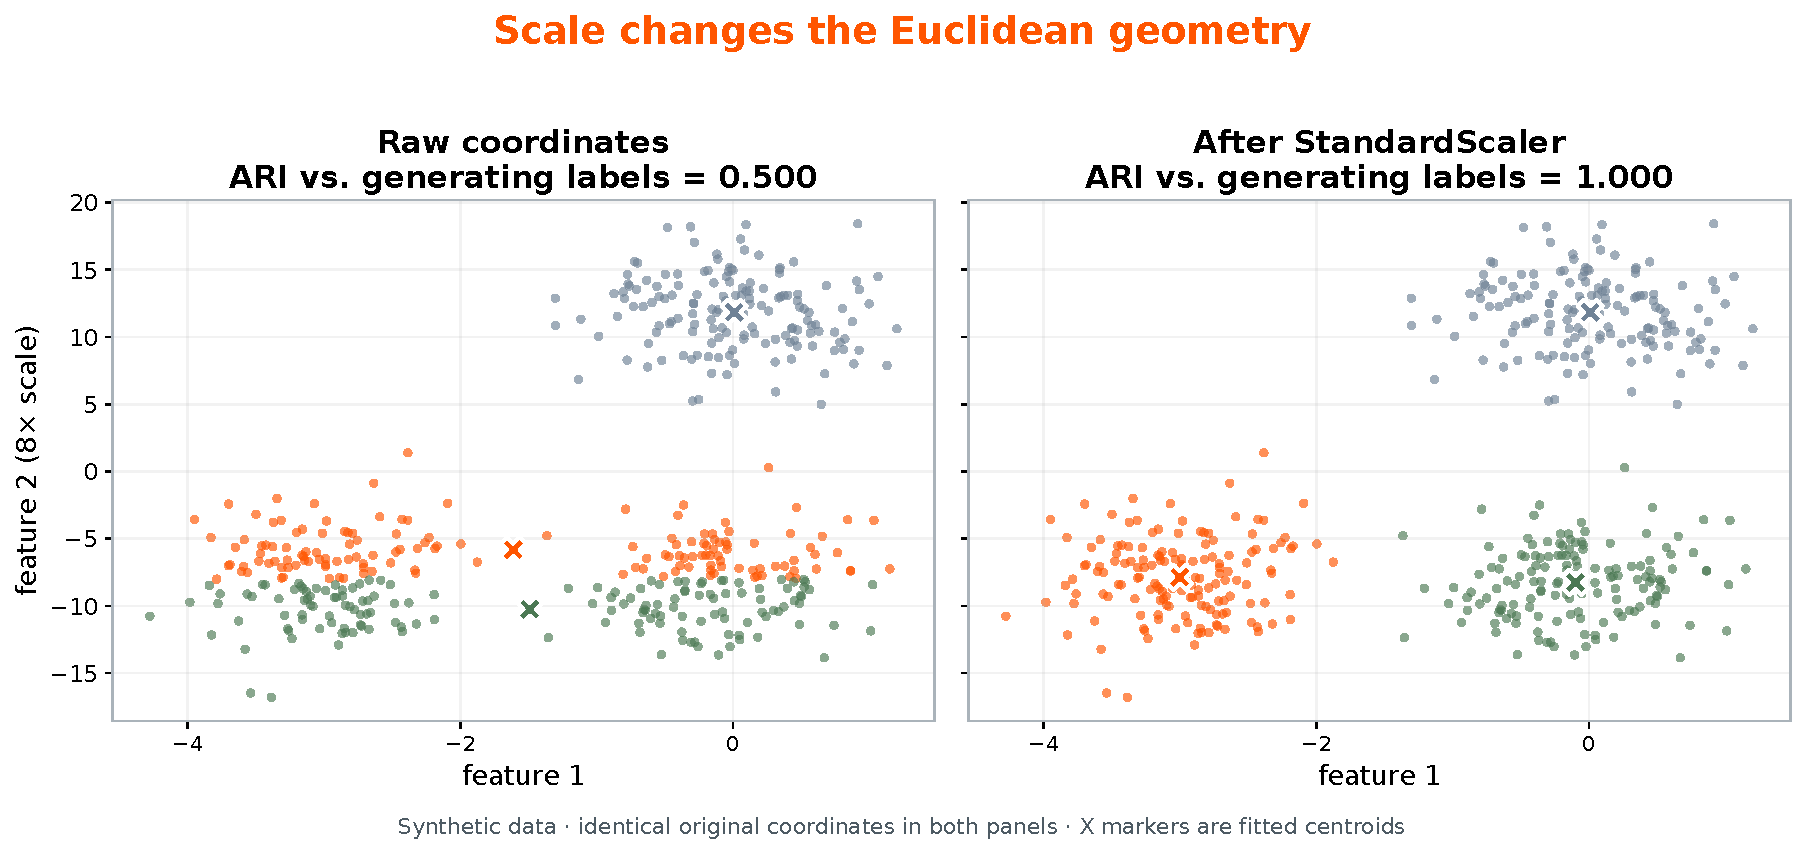
\includegraphics[width=.90\textwidth]{assets/fig_scale.pdf}
\end{frame}

% 21 --------------------------------------------------------------------------
\begin{frame}{Experiments Expose the Geometry Assumptions}
  \centering
  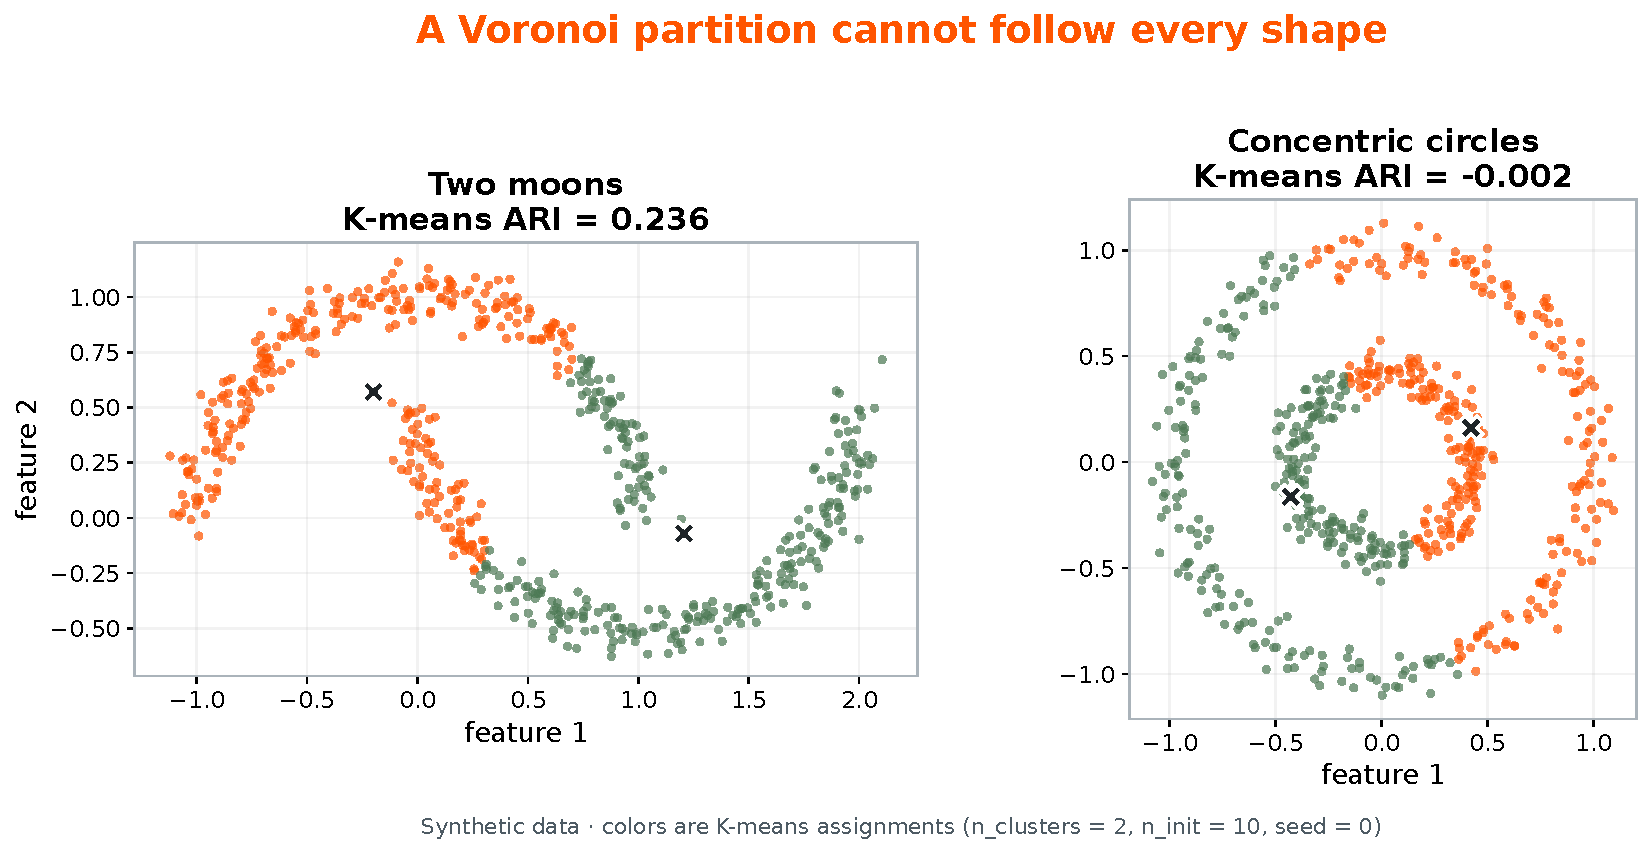
\includegraphics[width=.80\textwidth]{assets/fig_shape_failure.pdf}
\end{frame}

% 22 --------------------------------------------------------------------------
\begin{frame}{Remedies for the Non-regular Case}

      \textbf{Change the representation}
      \begin{itemize}\setlength{\itemsep}{.3cm}
        \item Engineer a radial feature, or use kernel K-means as an implicit nonlinear map.
        \item For concentric rings, $u=x_1^2+x_2^2$ is a radius coordinate.
        \item K-means on $u$ uses a one-dimensional threshold.
      \end{itemize}

  \vspace{.2cm}
  {\scriptsize\color{slideorange}\textbf{Challenge:} standard K-means does not train a feature map; the useful feature must come from data geometry or domain knowledge.}
\end{frame}

% 23 --------------------------------------------------------------------------


% 24 ------------------------------------------------------------------
% 25 --------------------------------------------------------------------------
\begin{frame}{A Practical Reporting Checklist}
  \begin{enumerate}\spaceditems
    \item State what one row $x$ represents and which features were used.
    \item Record scaling, transformations, missing-value handling, and distance.
    \item Run multiple initializations and report objective variability.
    \item Compare several $K$ values using internal and stability diagnostics.
    \item Inspect cluster sizes, profiles, and outliers.
    \item Keep labels or downstream outcomes for validation, not for fitting.
  \end{enumerate}
\end{frame}


\SectionSlideN{Distance-Preserving Reduction}

% 21 --------------------------------------------------------------------------
\begin{frame}{Random Projection Before K-means}
  \centering
  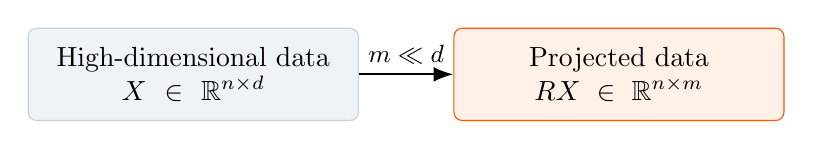
\begin{tikzpicture}[node distance=1.2cm]
    \node[softbox,text width=3.7cm] (high) {High-dimensional data\\$X\in\R^{n\times d}$};
    \node[orangebox,text width=3.7cm,right=of high] (low) {Projected data\\$RX\in\R^{n\times m}$};
    \draw[flow] (high)--node[above,font=\small]{$m\ll d$}(low);
  \end{tikzpicture}
  \vspace{.45cm}
  \begin{columns}[T,onlytextwidth]
    \column{.47\textwidth}
      \begin{itemize}\spaceditems
        \item Lower memory and distance-computation cost;
        \item useful when $d$ is much larger than $\log n$.
      \end{itemize}
    \column{.47\textwidth}
      \begin{itemize}\spaceditems
        \item Preserve sample geometry;
        \item projected coordinates need not be interpretable.
      \end{itemize}
  \end{columns}
  \pause
  \vspace{.2cm}
  \centering
  The question is whether the K-means objective survives the projection.
\end{frame}

% 22 --------------------------------------------------------------------------
\begin{frame}{Johnson--Lindenstrauss Lemma}
  For $n$ points and failure probability $\delta$, a random linear map
  $R:\R^d\to\R^m$ with
  \[
    m=O\!\left(\frac{\log(n/\delta)}{\varepsilon^2}\right)
  \]
  A common Gaussian-projection implementation uses the sufficient bound
  \[
    m\;\ge\;\frac{4\log n}{\varepsilon^2/2-\varepsilon^3/3}.
  \]
  can satisfy, simultaneously for every pair $i,j$,
  \[
    (1-\varepsilon)\norm{x_i-x_j}^2
    \le \norm{Rx_i-Rx_j}^2
    \le (1+\varepsilon)\norm{x_i-x_j}^2.
  \]
  \pause
  \vspace{0pt}
  
\begin{tikzpicture}
    \node[greenbox,text width=10.0cm,inner sep=2pt] {\small Typical choices: Gaussian entries scaled by $1/\sqrt m$, random signs, or a sparse random projection.};
  \end{tikzpicture}
\end{frame}

% 23 --------------------------------------------------------------------------
\begin{frame}{JL Preserve a K-means Cluster Cost}
  For a cluster $C$ with mean $\mu_C$,
  \[
    \sum_{i\in C}\norm{x_i-\mu_C}^2
    =\frac{1}{2|C|}\sum_{i,j\in C}\norm{x_i-x_j}^2.
  \]
  \pause
  After projection, the projected mean is $R\mu_C$, so
  \[
    \sum_{i\in C}\norm{Rx_i-R\mu_C}^2
    =\frac{1}{2|C|}\sum_{i,j\in C}\norm{Rx_i-Rx_j}^2.
  \]
  \pause
  \centering
  If JL preserves all pairwise distances, it preserves every fixed clustering cost within $1\pm\varepsilon$.
\end{frame}

% 24 --------------------------------------------------------------------------
\begin{frame}{The Projected Optimum Is Approximately Competitive}
  Let $C^*$ minimize the original K-means objective and $\widetilde C$ minimize the projected objective. For every partition $C$,
  \[
    (1-\varepsilon)J(C)\le J_R(C)\le(1+\varepsilon)J(C).
  \]
  \pause
  \begin{align*}
    J(\widetilde C)
    \le \frac{J_R(\widetilde C)}{1-\varepsilon}&\le \frac{J_R(C^*)}{1-\varepsilon}\le \frac{1+\varepsilon}{1-\varepsilon}J(C^*).
  \end{align*}
\end{frame}

% 25 -----------------------------------------------------------------------------------------------------------------------------


% 27 --------------------------------------------------------------------------
\begin{frame}{K-means in One Sentence}
  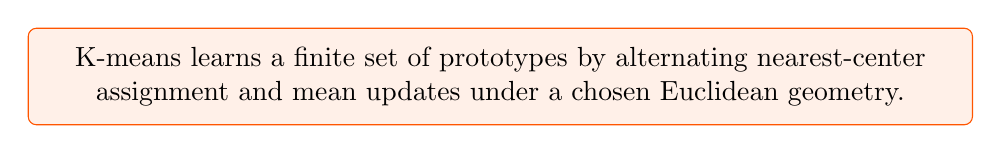
\begin{tikzpicture}
    \node[orangebox,text width=11.5cm,minimum height=1.2cm]
      {K-means learns a finite set of prototypes by alternating nearest-center assignment and mean updates under a chosen Euclidean geometry.};
  \end{tikzpicture}
  \vspace{.55cm}
  \begin{itemize}\spaceditems
    \item The objective explains the updates;
    \item the geometry explains the failure modes;
    \item initialization and preprocessing shape the result;
    \item evaluation must include stability and domain meaning;
    \item JL projection can reduce dimension while approximately preserving the objective.
  \end{itemize}
\end{frame}




\end{document}
